% !TEX program = xelatex
% 使用 ctexart文类,UTF-8 编码

\documentclass[openany,oneside]{midtermreport}

% 导言区,加载宏包和各项设置
% \usepackage{}
% 此处示意对参考文献和索引的设置

\begin{document}

% !Mode:: "TeX:UTF-8"

% ������Ӣ�ı���
\thesistitle
{����ʱ���������ݵ��ȴ�������̬�����о�}
{����ʱ���������ݵ��ȴ�������̬�����о�}
{Based on the Time-varying Meteorological Data of Tropical Cyclone Dynamic Simulation Research}
{Based on the Time-varying Meteorological Data of Tropical Cyclone Dynamic Simulation Research}


% !Mode:: "TeX:UTF-8"

% 学校名称 {中文}{英文}
\university{北京航空航天大学}{Beihang University}

% 院系英文名可从以下导航页面进入各个学院的主页查看
% http://www.buaa.edu.cn/xyykc/index.htm
\school
{计算机学院}{School of Computer Science and Engineering}

% 专业中英文名
\major
{计算机技术}{Computer Technology}

% 研究方向
\direction{虚拟现实技术}{Virtual Reality Technology}

% 论文提交时间
\commit{2012}{03}{03}

% 学生学号
\studentid{ZY1406204}

% 论文作者
\thesisauthor
{李阳}{Li Yang}

% 导师中英文名
\teacher
{齐越}{Qi Yue}

\tercher


    
\maketitle % 封面页眉页脚页码样式

% 目录页眉页脚页码样式
\pagestyle{frontmatter}% 前言页眉页脚样式
\tableofcontents

% 正文页眉页脚页码样式
\mainmatter

\pagestyle{mainmatter} % 正文页眉页脚样式
\relaxclearpage
\printtitle
% !TEX root = ../midtermreport.tex
% !Mode:: "TeX:UTF-8"

\chapter{论文工作计划}
\label{chap:research_plan}

\section{论文研究目标}
\label{sect:research_goal}

% 介绍热带气旋
本论文主要研究一种常见的天气现象---热带气旋的模拟与仿真技术。
热带气旋(Tropical Cyclone,简称TC)
指的是一种快速旋转的风暴天气系统,有一个低气压中心和螺旋结构的云体,
同时伴随着强风、雷电、暴雨等现象,也被称作台风、飓风、热带风暴、气旋风暴、热带低压等。
一个成熟的热带气旋通常有完整的结构,其结构如图\ref{fig:tc_structure}所示,主要包括风眼,地面低压,暖心,中心密集云层区,风眼墙,螺旋雨带,外散环流等构成。
\begin{figure}[h!]
	\centering
	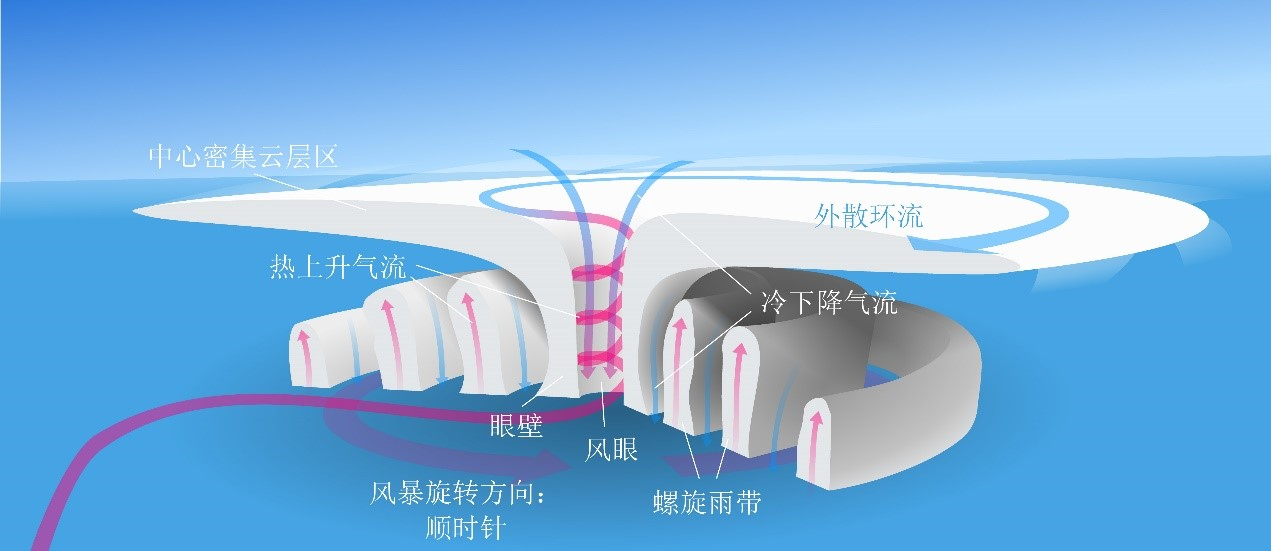
\includegraphics[width=400bp]{figure/tcstructure.jpg}
	\caption{热带气旋结构图}
	\label{fig:tc_structure}
\end{figure}

% 介绍研究意义
热带气旋的模拟和仿真技术一直是气象、海洋等领域演技研究的重点和难点,
而在计算机图形图像学领域,由于其独特的结构,热带气旋也是作为一个重要的研究内容。
其中主要包括研究热带气旋的可视化效果,云的真实感绘制技术,以及热带气旋的模拟技术。
同时能够较真实的模拟热带气旋的运动以及真实的展现其结构,
对气象研究、海洋研究、气象预测等具有极其重要的意义。

% 研究现状
在计算机图形图形领域,对热带气旋方面的的研究主要集中在对云的建模和仿真。
随着虚拟场景渲染技术的发展,云的模拟表现也成为计算机图形学和虚拟现实技术中的热门课题。
云的真实感模拟不仅能有效提高场景逼真度,更能传达丰富的气象信息。
云作为一种常见的自然现象,由于其形状千变万化,形成、发展和消散的过程又极其复杂,
且具有水汽粒子的半透明特征。
能够实现即满足气象学应用,同时实现逼真展现的云场景模拟是一项很艰巨的任务。

早期在图形图像学领域云建模大体分为两类,
即基于过程的云建模和基于物理的云建模。
前者侧重于利用噪声、纹理或者交互式的手段对云进行建模,通常需要经历繁琐的参数调整;
后者则通过求解简化的NS方程,模拟云生成的物理过程,
这种方法耗时大,且不能有效生成预期形状的云。

基于数据驱动的云建模,在一定程度上能够克服之前建模方法的缺点,
且由于其建模过程中参考了真实数据,
能够在一定程度上反映数据信息、表达气象属性,因此具有很强的应用意义,逐渐成为研究的热点。
通过研究和分析云的相关数据(自然图像、观测数据、数值模拟数据、卫星云图等),
进一步从数据中发掘能够指导云建模的信息,
构建逼真的三维云场,同时与真实数据在形状、气象信息、规模上具有一定相关性。
相应的成果可以为天气数值预测、军事仿真、卫星气象等领域提供可视化工具和环境。

% 本论文的意义
基于时变气象数据的热带气旋的仿真技术,相比于传统的图形图像学建模方法,
由于使用的是数值模拟数据(Weather Research and Forecasting Model,简称WRF)进行建模,
模型本身就具有真实性,同时通过时序数据的矫正,使得仿真的数据气象学的意义,
符合气象学用户对数据准确性的要求;
同时又在时域内使用简单NS方程模拟云的运动过程,使得模拟速度能够达到实时应用的需求。

综述所述,热带气旋仿真技术具重要的研究意义以及广阔的应用前景,
但是现有方法建模过程难以实现及满足气象需求,同时满足逼真展现的应用。
因此,本文提出的仿真方法具有重要的意义。

% 研究目标
本论文的研究目标:针对热带气旋这一种复杂的天气系统,
设计并实现一个热带气旋的动态仿真模拟算法。 
该算法使用气象数据做初始状态,同时以长时间跨度的时变气象数据为输入,
使用基于位置的流体仿真(position based Fluids,简称PBF)方法,利用GPU加速计算云的仿真,
输出指定时间跨度的粒子数据,在保留更多细节的同时,保证仿真过度自然流畅。

在此基础上,结合基于粒子的云建模方法和
基于粒子系统的LOD(Level of Detail)层级结构的绘制方法,
形成包括建模、仿真、绘制的热带气旋动态仿真系统。

\section{论文主要研究内容}

本论文的主要研究内容包括:
提取WRF数据中的云相关建模参量建立云的粒子模型,
根据使用PBF仿真技术模拟云的运动过程,
根据WRF数据中的每一帧数据,校正PBF流体仿真产生的误差,
最后基于粒子系统的LOD层级结构,使用多散射模型的绘制方法绘制具有真实感的云。
流程图如图\ref{fig:research_contents}

本论文主要研究的内容如图\ref{fig:research_contents}所示,该图给出了整个系统的模块划分和模块之间的输入输出关系。具体内容阐述如下:
\begin{figure}[h!]
	\centering
	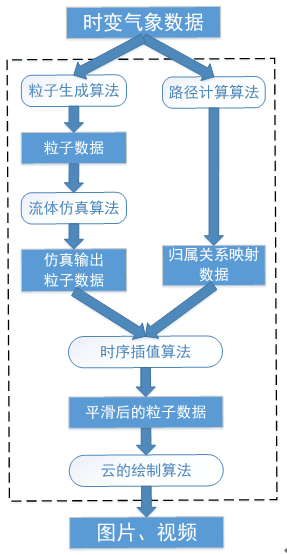
\includegraphics[width = 150bp]{figure/researchContemts.png}
	\caption{基于时变气象数据的热带气旋动态仿真技术研究流程图}
	\label{fig:research_contents}
\end{figure}

\begin{enumerate}

\item \textbf{基于WRF数据的云粒子建模}

粒子构建算法是将给予欧拉表征的时变气象数据通过插值、
采样等方法构建基于拉格朗日表征的差分粒子结构数据。
目的是能够更好的表示热带气旋的表观结构,
同时有利于后面的流体仿真和时序插值计算。

\item \textbf{PHF流体仿真}

流体仿真算法是本课题的一个重点研究内容,
其输入是流体的初始状态,输出为后续若干时刻的流体状态。
本题目主要的功能是进行有物理意义的长时间跨度的插值,
如果仅使用基于图形图像方面的插值算法,
会导致插值的数据不具有物理意义,不够真实。
同时对云的真实感绘制如果没有流体仿真技术的应用,
也就不具有其真实感的含义。

\item \textbf{路径计算算法}

路径计算算法的输入时气象数据的速度场数据,其输出是粒子与流线归属关系映射数据结构。
路径计算算法实现的不只是路劲的计算,同时还有实现归属映射关系的构建。
流线的生成是为了使粒子的位置完全覆盖当前时刻所有非零密度点流体的体积的同时
用尽可能少的粒子完成紧凑的计算。
构造粒子与流线归属关系的映射,为后面的误差校准提供参考依据。

\item \textbf{时序插值算法}

时序插值算法的输入时经过流体仿真输出的粒子数据和经过路径计算求得的归属关系,
输出是经过插值的粒子数据。该算法是本课题的难点。
众所周知,通过流体仿真计算得到的数据,到达下一时刻时与原数据之间是不能保持一致的,
原因就在NS方程表达的函数与我们仿真的函数是有差别的,而这种差别是不可能避免的。
因此还需要一个基于流体仿真的时序插值算法去实现流体的平滑过渡。

\item \textbf{云的绘制算法}

云的绘制算法的输入是经过平滑处理后的粒子数据,输出是仿真展现的画面。
通过以上的动态仿真,得到相应的数据,通过绘制系统绘制展现出来。
由于热带气旋属于大中尺度的天气现象,针对这种大尺度的云绘制,
一方面要实现光照的计算,同时要对大量粒子的事实绘制,云的绘制已是一个重要的研究点。

\end{enumerate}



 % 第一章chapter1.tex
% !Mode:: "TeX:UTF-8"
\chapter{已经完成的工作}

\section{C\TeX{}套装 [Windows Only]}

C\TeX{}套装是Windows下为中文优化的\LaTeX{}系统套件,主要基于MiKTeX系统,
集成了编辑器WinEdt和其他相关软件。整个系统封装在一个安装程序中,
安装方法与常规软件相同,无需任何配置,适合大部分Windows用户使用。

\begin{description}
    \item[下载地址] \hfill
    \begin{description}
        \item[官方页面]
            \url{http://www.ctex.org/CTeXDownload}
        \item[未来花园]
            稍后我们也会提供未来花园上的下载页面,敬请关注
    \end{description}
    \item[安装方法] \hfill
        \begin{itemize}
            \item[] 与常规软件的安装方法差不多
            \item[] 一直下一步稍加一些自定义(如安装路径)即可
        \end{itemize}
\end{description}

\section{\TeX{}Live [ Windows \& Linux ]}

\TeX{}是自由软件,有很多发行版本,就像Linux的Ubuntu、Fedora等等。
每个发行版本都是一套工具集合,包括plain\TeX{},\LaTeX{},pdf\TeX{},dvips等。
其中比较流行的是\TeX{}Live,也包含在CTAN的开源镜像中,
目前的最新版本是\TeX{}Live 2012。

推荐通过下载ISO镜像文件的方式安装:
\begin{description}
    \item[官方说明]
        \url{http://www.tug.org/texlive/acquire-iso.html}
    \item[下载地址] 官方地址会自动跳转寻找"最近"镜像,还有几个较快的教育网镜像
    \begin{description}
        \item[官方地址]
            \url{http://mirror.ctan.org/systems/texlive/Images/texlive2012.iso}
        \item[清华镜像]
            \url{http://mirrors.tuna.tsinghua.edu.cn/CTAN/systems/texlive/Images/}
        \item[北交镜像]
            \url{http://mirror.bjtu.edu.cn/CTAN/systems/texlive/Images/}
        \item[未来花园]
            稍后我们也会提供未来花园上的下载页面,敬请关注
    \end{description}
    \item[安装方法] \hfill
    \begin{enumerate}
        \item 通过虚拟光驱挂载镜像也可以直接打开或解压缩不过会比较慢
        \item 双击运行光盘镜像或者运行脚本
        \item[] Windows 用户可以直接双击运行\textsl{install-tl.bat}
        \item[] Linux 用户可以在终端下执行命令\textsl{./install-tl}
        \item 按照提示下一步即可,安装大致耗时10$\sim$20分钟,受机器配置影响。
    \end{enumerate}
\end{description}

当然官方也提供了通过网络安装的方式,虽然通过可以通过镜像选择达到比较快的速度,
但是这里简便期间不再赘述,有兴趣的同学可以参考官方说明
\url{http://www.tug.org/texlive/acquire-netinstall.html}。

\section{Mac\TeX{} [ Mac ]}

Mac\TeX{}是基于\TeX{}Live为Mac系统设计的套件。

\begin{description}
    \item[官方网站]
        \url{http://tug.org/mactex/}
    \item[下载地址] 官方地址会自动跳转寻找"最近"镜像,还有几个较快的教育网镜像
    \begin{description}
        \item[官方地址]
            \url{http://mirror.ctan.org/systems/mac/mactex/MacTeX.pkg}
        \item[清华镜像]
            \url{http://mirrors.tuna.tsinghua.edu.cn/CTAN/systems/mac/mactex/}
        \item[北交镜像]
            \url{http://mirror.bjtu.edu.cn/CTAN/systems/mac/mactex/}
        \item[未来花园]
            稍后我们也会提供未来花园上的下载页面,敬请关注
    \end{description}
    \item[安装方法] 同一般软件安装,下一步即可
\end{description}

\section{关于编辑器}

以上介绍了三款\LaTeX{}套装,涵盖了主流的三大平台,除了C\TeX{}自带了WinEdt,
其余两款均需要自己选择编辑器,理论上任何文本编辑器都是可以使用的,
如Windows上的Notepad++,Linux/MacOS上的vim,emacs,
一方面要考虑对\LaTeX{}的支持,一方面还是自己的熟悉程度。

这里推荐一款大众化的编辑器\TeX{}maker,它是跨平台的,支持Windows、Linux和MacOS。

\begin{description}
    \item[官方网站]
        \url{http://www.xm1math.net/texmaker/}
    \item[下载地址]
        \url{http://www.xm1math.net/texmaker/download.html}
    \item[相关说明]
    \begin{itemize}
        \item 安装同一般软件的安装
        \item 配置Xe\LaTeX{}的编译,选择菜单栏“选项”->“配置\TeX{}Maker”,
        \item[] 在“\LaTeX{}”一栏填写
            \texttt{xelatex -interaction=nonstopmode\%.tex}
    \end{itemize}
\end{description}

\section{关于编译}

\LaTeX{}的文件是通过编译生成的,对于本模板和毕业设计论文而言,
需要经过代码\ref{code-compile}所示步骤(以sample-bachelor.tex为例):
\begin{lstlisting}[
    language={bash},
    caption={编译步骤},
    label={code-compile},
]
xelatex sample-bachelor.tex
bibtex  sample-bachelor.aux
xelatex sample-bachelor.tex
xelatex sample-bachelor.tex
\end{lstlisting}
当然,我们在模板里也提供了编译的执行脚本。

\subsection{批处理 [ Windows only ]}

进入cmd(Win+R,然后输入cmd),cd到BUAAthesis对应目录,
如{\verb D:\BUAAthesis\ },然后运行{\verb msmake }即可。

\subsection{Makefile [ Windows(cygwin) / Linux / MacOS ]}
需要要你的命令行环境支持Make,cd到BUAAthesis相应目录,
目前支持如代码\ref{code-make}所示的功能:
\begin{lstlisting}[
    language={bash},
    caption={make 命令},
    label={code-make},
]
make bachelor # 编译本科生的\LaTeX{}(文件默认项,亦可直接输入make)
make master # 编译研究生的\LaTeX{}文件
make clean # 删除编译过程中生成的文件(除了pdf)
make depclean # 删除编译过程中生成的文件(包括pdf)
\end{lstlisting}
 % 第二章chapter1.tex
% !Mode:: "TeX:UTF-8"
\chapter{关键技术和难点}

\section{发行版本}

发行版本是本模板编写者会不定期更新打包的版本,适合大部分用户使用,
优点是相对较为稳定,下载和使用都更方便便捷,
缺点是可能不包含一些最新的更新,不过应该足够满足常规毕业设计论文撰写需求。
由于本模板仍在开发之中,我们将适时更新本说明文档及相关项目介绍和使用方法,
敬请关注后续进展。

\section{开发版本}

开发版本是通过Git直接clone本模板托管在Github版本库中的最新代码,
适合有版本管理工具使用经验和对LaTeX使用较为熟练的用户。
优点是包含最新的模板代码,
缺点是稳定性无法保证,可能有一些小问题,
当然我们很欢迎您通过所有可能的方式将问题反馈给我们。

\subsection{下载方法}
首先你需要打开准备存放毕业设计论文的目录,
通过命令\ref{code-git-clone}即可获取最新的模板代码,
需要注意的是这将在当前目录下新建一个名为BUAAthesis的文件夹。
\begin{lstlisting}[
    language={bash},
    caption={git clone},
    label={code-git-clone},
]
git clone git://github.com/BHOSC/BUAAthesis.git
\end{lstlisting}

\subsection{更新方法}
通过命令\ref{code-git-pull}即可实现模板代码的更新,
需要注意的是此处可能会出现冲突,相关处理方法将在后续说明。
\begin{lstlisting}[
    language={bash},
    caption={git pull},
    label={code-git-pull},
]
git pull origin master
\end{lstlisting}

\section{目录结构}

本模板项目完整的文件目录结构如下所示:

{
    \dirtree{%
        .1 BUAAthesis/\DTcomment{根目录}.
        .2 buaathesis.cls\DTcomment{模板文件}.
        .2 buaathesis.bst\DTcomment{参考文献样式}.
        .2 sample-bachelor.tex\DTcomment{本科生示例文件}.
        .2 sample-master.tex\DTcomment{研究生示例文件}.
        .2 data/\DTcomment{数据文件夹}.
        .3 abstract.tex\DTcomment{中英文摘要}.
        .3 appendix1-faq.tex\DTcomment{附录1,常见问题}.
        .3 appendix2-contactus.tex\DTcomment{附录2,联系我们}.
        .3 bibs.bib\DTcomment{参考文献文件}.
        .3 chapter1-intro.tex.
        .3 chapter2-config.tex.
        .3 chapter3-download.tex.
        .3 chapter4-baisc.tex.
        .3 chapter5-usage.tex.
        .3 chapter6-implement.tex.
        .3 com\_info.tex\DTcomment{通用自定义信息}.
        .3 reference.tex\DTcomment{参考文献}.
        .3 bachelor/\DTcomment{本科生专属文件}.
        .4 assign.tex\DTcomment{任务书}.
        .4 bachelor\_info.tex\DTcomment{本科生专属信息}.
        .4 acknowledgement.tex\DTcomment{致谢页}.
        .3 master/\DTcomment{研究生专属文件}.
        .4 back1-achievement.tex\DTcomment{附页1,取得成绩}.
        .4 back2-acknowledgement.tex\DTcomment{附页2,致谢}.
        .4 back3-aboutauthor.tex\DTcomment{附页3,关于作者}.
        .4 denotation.tex\DTcomment{主要符号对照表}.
        .4 master\_info.tex\DTcomment{研究生专属信息}.
        .2 figure/\DTcomment{图片存放路径}.
        .3 buaamark.eps\DTcomment{北航Logo,用于页眉}.
        .3 buaaname.eps\DTcomment{北航校名,用于首页}.
        .3 fgbt.jpg\DTcomment{北航未来花园Logo,用于测试}.
        .2 Makefile\DTcomment{Linux下辅助脚本}.
        .2 msmake.bat\DTcomment{Windows下辅助脚本}.
        .2 README.md\DTcomment{Github项目说明}.
        .2 .gitignore\DTcomment{Git版本管理配置文件}.
    }
}
 % 第三章chapter1.tex
% !TEX root = ../midtermreport.tex
% !Mode:: "TeX:UTF-8"
\chapter{下一阶段工作计划}
\label{chap:next}


\section{尚未完成的工作}
	本论文尚未完全完成的工作包括
	
\begin{enumerate}
	\item 仿真过程过的校正
	\item 系统的完善和集成
	\item 系统全面的功能性测试
	\item 毕业设计论文的撰写
\end{enumerate}
\section{存在的问题}

目前实验效果已经能够完成时序数据的建模和插值过程,但存在两个时间帧数据的平滑过渡问题,
即存在两帧数据之间发生跳变现象,这也是目前没有完全克服的问题,
还需在下一步工作中设计改进方案。

\section{解决问题的技术思路或措施}
目前已经基本实现光滑过度,但还存在存在一些瑕疵,下一步考虑引入后向插值技术,校正模拟结果,
对仿真过程进行完善。
\section{下一阶段计划}

\begin{enumerate}
	\item 8月至9月,仿真过程过的校正
	\item 9月至10月,系统集成和测试
	\item 10月至12月,撰写毕业论文	
\end{enumerate}




 % 第二章chapter2.tex

% !TEX root = ../midtermreport.tex
% !Mode:: "TeX:UTF-8"
\cleardoublepage
\phantomsection
\chapter{主要参考文献}
\nocite{*}
\bibliography{data/bibs}
\cleardoublepage
 % 第二章chapter2.tex

\end{document}